\documentclass[]{article}
\usepackage{lmodern}
\usepackage{amssymb,amsmath}
\usepackage{ifxetex,ifluatex}
\usepackage{fixltx2e} % provides \textsubscript
\ifnum 0\ifxetex 1\fi\ifluatex 1\fi=0 % if pdftex
  \usepackage[T1]{fontenc}
  \usepackage[utf8]{inputenc}
\else % if luatex or xelatex
  \ifxetex
    \usepackage{mathspec}
  \else
    \usepackage{fontspec}
  \fi
  \defaultfontfeatures{Ligatures=TeX,Scale=MatchLowercase}
\fi
% use upquote if available, for straight quotes in verbatim environments
\IfFileExists{upquote.sty}{\usepackage{upquote}}{}
% use microtype if available
\IfFileExists{microtype.sty}{%
\usepackage{microtype}
\UseMicrotypeSet[protrusion]{basicmath} % disable protrusion for tt fonts
}{}
\usepackage[margin=1in]{geometry}
\usepackage{hyperref}
\hypersetup{unicode=true,
            pdfborder={0 0 0},
            breaklinks=true}
\urlstyle{same}  % don't use monospace font for urls
\usepackage{color}
\usepackage{fancyvrb}
\newcommand{\VerbBar}{|}
\newcommand{\VERB}{\Verb[commandchars=\\\{\}]}
\DefineVerbatimEnvironment{Highlighting}{Verbatim}{commandchars=\\\{\}}
% Add ',fontsize=\small' for more characters per line
\usepackage{framed}
\definecolor{shadecolor}{RGB}{248,248,248}
\newenvironment{Shaded}{\begin{snugshade}}{\end{snugshade}}
\newcommand{\KeywordTok}[1]{\textcolor[rgb]{0.13,0.29,0.53}{\textbf{#1}}}
\newcommand{\DataTypeTok}[1]{\textcolor[rgb]{0.13,0.29,0.53}{#1}}
\newcommand{\DecValTok}[1]{\textcolor[rgb]{0.00,0.00,0.81}{#1}}
\newcommand{\BaseNTok}[1]{\textcolor[rgb]{0.00,0.00,0.81}{#1}}
\newcommand{\FloatTok}[1]{\textcolor[rgb]{0.00,0.00,0.81}{#1}}
\newcommand{\ConstantTok}[1]{\textcolor[rgb]{0.00,0.00,0.00}{#1}}
\newcommand{\CharTok}[1]{\textcolor[rgb]{0.31,0.60,0.02}{#1}}
\newcommand{\SpecialCharTok}[1]{\textcolor[rgb]{0.00,0.00,0.00}{#1}}
\newcommand{\StringTok}[1]{\textcolor[rgb]{0.31,0.60,0.02}{#1}}
\newcommand{\VerbatimStringTok}[1]{\textcolor[rgb]{0.31,0.60,0.02}{#1}}
\newcommand{\SpecialStringTok}[1]{\textcolor[rgb]{0.31,0.60,0.02}{#1}}
\newcommand{\ImportTok}[1]{#1}
\newcommand{\CommentTok}[1]{\textcolor[rgb]{0.56,0.35,0.01}{\textit{#1}}}
\newcommand{\DocumentationTok}[1]{\textcolor[rgb]{0.56,0.35,0.01}{\textbf{\textit{#1}}}}
\newcommand{\AnnotationTok}[1]{\textcolor[rgb]{0.56,0.35,0.01}{\textbf{\textit{#1}}}}
\newcommand{\CommentVarTok}[1]{\textcolor[rgb]{0.56,0.35,0.01}{\textbf{\textit{#1}}}}
\newcommand{\OtherTok}[1]{\textcolor[rgb]{0.56,0.35,0.01}{#1}}
\newcommand{\FunctionTok}[1]{\textcolor[rgb]{0.00,0.00,0.00}{#1}}
\newcommand{\VariableTok}[1]{\textcolor[rgb]{0.00,0.00,0.00}{#1}}
\newcommand{\ControlFlowTok}[1]{\textcolor[rgb]{0.13,0.29,0.53}{\textbf{#1}}}
\newcommand{\OperatorTok}[1]{\textcolor[rgb]{0.81,0.36,0.00}{\textbf{#1}}}
\newcommand{\BuiltInTok}[1]{#1}
\newcommand{\ExtensionTok}[1]{#1}
\newcommand{\PreprocessorTok}[1]{\textcolor[rgb]{0.56,0.35,0.01}{\textit{#1}}}
\newcommand{\AttributeTok}[1]{\textcolor[rgb]{0.77,0.63,0.00}{#1}}
\newcommand{\RegionMarkerTok}[1]{#1}
\newcommand{\InformationTok}[1]{\textcolor[rgb]{0.56,0.35,0.01}{\textbf{\textit{#1}}}}
\newcommand{\WarningTok}[1]{\textcolor[rgb]{0.56,0.35,0.01}{\textbf{\textit{#1}}}}
\newcommand{\AlertTok}[1]{\textcolor[rgb]{0.94,0.16,0.16}{#1}}
\newcommand{\ErrorTok}[1]{\textcolor[rgb]{0.64,0.00,0.00}{\textbf{#1}}}
\newcommand{\NormalTok}[1]{#1}
\usepackage{graphicx,grffile}
\makeatletter
\def\maxwidth{\ifdim\Gin@nat@width>\linewidth\linewidth\else\Gin@nat@width\fi}
\def\maxheight{\ifdim\Gin@nat@height>\textheight\textheight\else\Gin@nat@height\fi}
\makeatother
% Scale images if necessary, so that they will not overflow the page
% margins by default, and it is still possible to overwrite the defaults
% using explicit options in \includegraphics[width, height, ...]{}
\setkeys{Gin}{width=\maxwidth,height=\maxheight,keepaspectratio}
\IfFileExists{parskip.sty}{%
\usepackage{parskip}
}{% else
\setlength{\parindent}{0pt}
\setlength{\parskip}{6pt plus 2pt minus 1pt}
}
\setlength{\emergencystretch}{3em}  % prevent overfull lines
\providecommand{\tightlist}{%
  \setlength{\itemsep}{0pt}\setlength{\parskip}{0pt}}
\setcounter{secnumdepth}{0}
% Redefines (sub)paragraphs to behave more like sections
\ifx\paragraph\undefined\else
\let\oldparagraph\paragraph
\renewcommand{\paragraph}[1]{\oldparagraph{#1}\mbox{}}
\fi
\ifx\subparagraph\undefined\else
\let\oldsubparagraph\subparagraph
\renewcommand{\subparagraph}[1]{\oldsubparagraph{#1}\mbox{}}
\fi

%%% Use protect on footnotes to avoid problems with footnotes in titles
\let\rmarkdownfootnote\footnote%
\def\footnote{\protect\rmarkdownfootnote}

%%% Change title format to be more compact
\usepackage{titling}

% Create subtitle command for use in maketitle
\providecommand{\subtitle}[1]{
  \posttitle{
    \begin{center}\large#1\end{center}
    }
}

\setlength{\droptitle}{-2em}

  \title{}
    \pretitle{\vspace{\droptitle}}
  \posttitle{}
    \author{}
    \preauthor{}\postauthor{}
    \date{}
    \predate{}\postdate{}
  

\begin{document}

knitr--- title: ``TDDE07 - Lab 1'' author: - ``Arvid Edenheim -
arved490'' - ``Sophie Lindberg - sopli268'' date: ``2019-04-13'' output:
pdf\_document header-includes: \usepackage{float}
\floatplacement{figure}{H} ---

\newpage

\section{1. Bernoulli \ldots{} again}\label{bernoulli-again}

\subsection{1a)}\label{a}

The posterior converges towards the true values with rising number of
draw, represented below with 10, 100, 1000 draws.

\begin{figure}
\centering
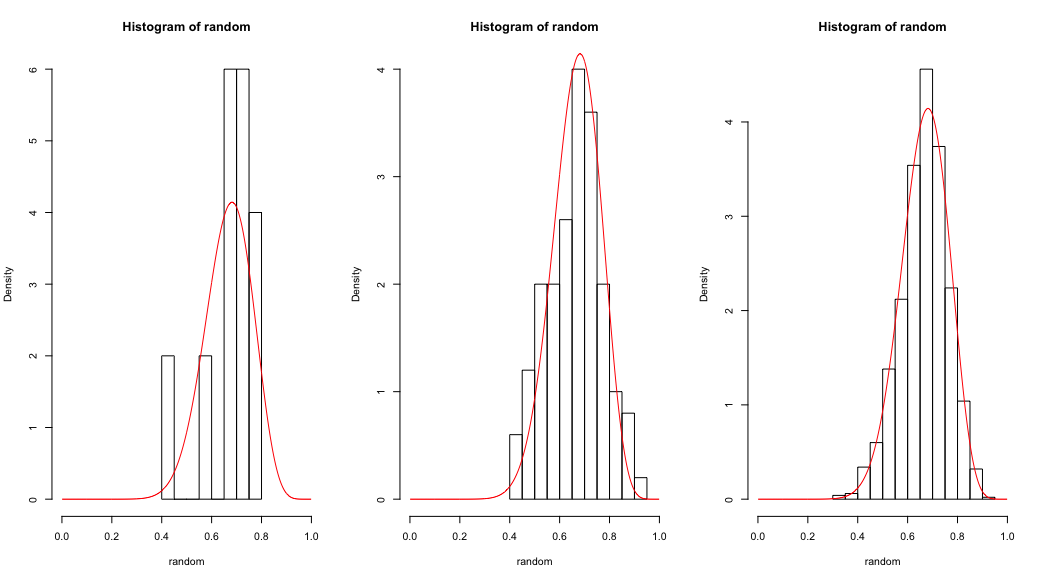
\includegraphics{assets/lab_1_1_a.png}
\caption{Convergence}
\end{figure}

\subsection{1b)}\label{b}

The posterior was simulated with 10000 draws, resulting in
\(P(\theta < 0.4 | y) = 0.0043\). Real value using pbeta = 0.003973.

\newpage

\subsection{1c)}\label{c}

Visualization of the log odds \(\phi = log(\frac{\phi}{1-\phi})\) by
simulation, using 10000 draws.

\begin{figure}
\centering
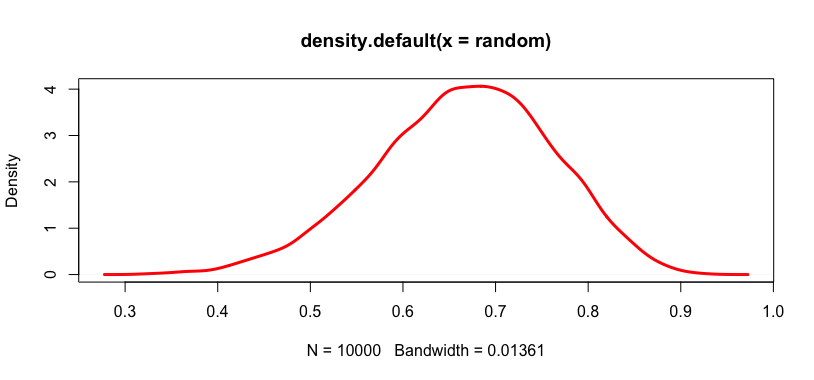
\includegraphics{assets/lab_1_1_c.png}
\caption{Posterior distribution of the log-odds}
\end{figure}

\newpage

\section{2. Log-normal distribution and the Gini
coefficient}\label{log-normal-distribution-and-the-gini-coefficient}

\subsection{2a)}\label{a-1}

Simulation of the posterior distribution of \(\sigma^{2}\) with 10,000
draws (histogram) compared to the theoretical distribution (line).'

\begin{figure}
\centering
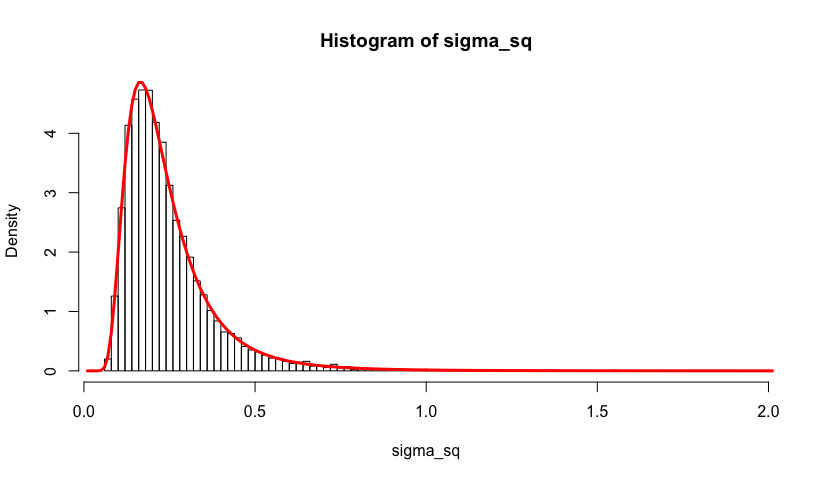
\includegraphics{assets/lab_1_2_a.png}
\caption{Posterior of \(\sigma^{2}\) by draws and the theoretical
posterior}
\end{figure}

\newpage

\subsection{2b)}\label{b-1}

The posterior distribution of the Gini coefficient based on the draws in
a).

\begin{figure}
\centering
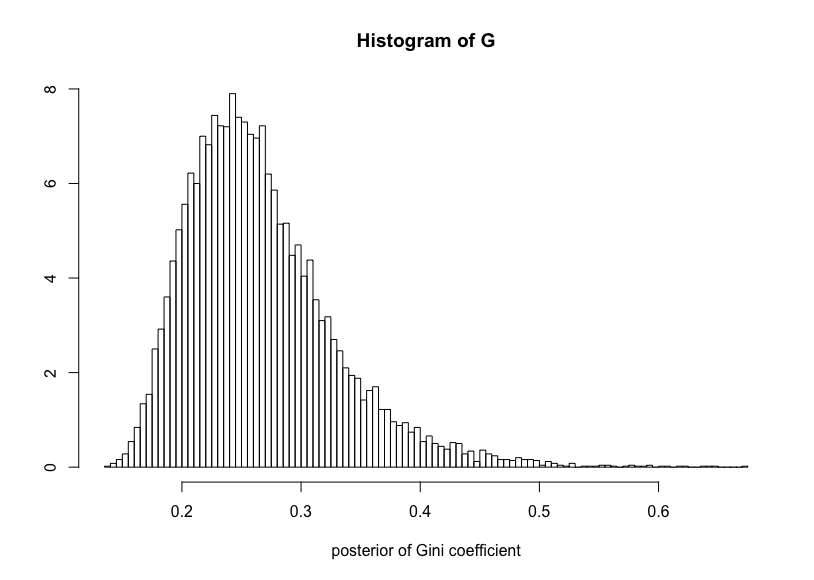
\includegraphics{assets/lab_1_2_b.png}
\caption{Gini Coefficient}
\end{figure}

\newpage

\subsection{2c)}\label{c-1}

Due to the long right tail, the Equal Tail Interval was slightliy
shifted to the right. The Highest Posterior Density interval produced a
better representatition of the data.

\begin{figure}
\centering
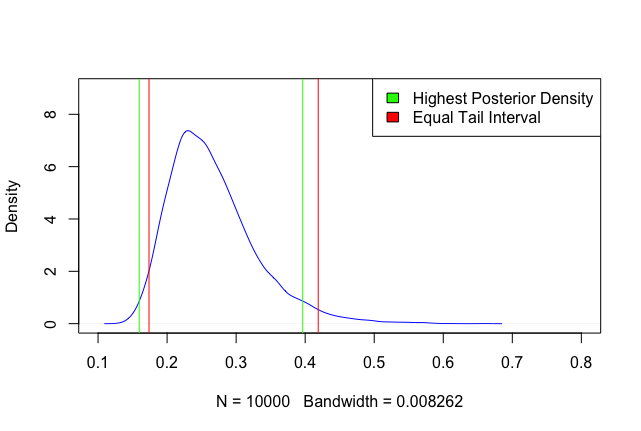
\includegraphics{assets/lab_1_2_c.png}
\caption{95\% Credibility interval}
\end{figure}

\newpage

\section{3. Bayesian inference for the concentration parameter in the
von Mises
distribution}\label{bayesian-inference-for-the-concentration-parameter-in-the-von-mises-distribution}

The distribution of \(\kappa\) was calculated as the product of the
likelihood and the prior, where the likelihood was assumed to be the
product of the individual probabilities due to independent observations.

\begin{figure}
\centering
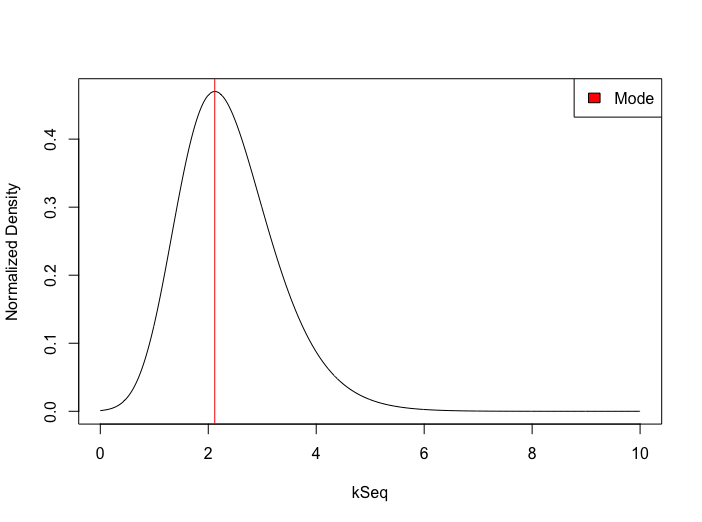
\includegraphics{assets/lab_1_3_ab.png}
\caption{Posterior distribution and mode}
\end{figure}

\newpage

\section{1 - Code}\label{code}

\begin{Shaded}
\begin{Highlighting}[]
\NormalTok{alpha <-}\StringTok{ }\DecValTok{2}
\NormalTok{beta <-}\StringTok{ }\DecValTok{2}
\NormalTok{s <-}\StringTok{ }\DecValTok{14}
\NormalTok{n <-}\StringTok{ }\DecValTok{20}
\NormalTok{nDraws <-}\StringTok{ }\KeywordTok{c}\NormalTok{(}\DecValTok{10}\NormalTok{, }\DecValTok{100}\NormalTok{, }\DecValTok{1000}\NormalTok{)}

\CommentTok{# 1a}

\NormalTok{xGrid <-}\StringTok{ }\KeywordTok{seq}\NormalTok{(}\FloatTok{0.001}\NormalTok{, }\FloatTok{0.999}\NormalTok{, }\DataTypeTok{by=}\FloatTok{0.001}\NormalTok{)}
\NormalTok{posterior =}\StringTok{ }\KeywordTok{dbeta}\NormalTok{(xGrid, alpha }\OperatorTok{+}\StringTok{ }\NormalTok{s, beta }\OperatorTok{+}\StringTok{ }\NormalTok{(n}\OperatorTok{-}\NormalTok{s))}
\KeywordTok{par}\NormalTok{(}\DataTypeTok{mfrow=}\KeywordTok{c}\NormalTok{(}\DecValTok{1}\NormalTok{,}\DecValTok{3}\NormalTok{))}
\ControlFlowTok{for}\NormalTok{ (draws }\ControlFlowTok{in}\NormalTok{ nDraws) \{}
\NormalTok{  random =}\StringTok{ }\KeywordTok{rbeta}\NormalTok{(draws, alpha}\OperatorTok{+}\NormalTok{s, beta}\OperatorTok{+}\NormalTok{(n}\OperatorTok{-}\NormalTok{s))}
  \KeywordTok{hist}\NormalTok{(random, }\DataTypeTok{xlim =} \KeywordTok{c}\NormalTok{(}\DecValTok{0}\NormalTok{,}\DecValTok{1}\NormalTok{), }\DataTypeTok{freq =} \OtherTok{FALSE}\NormalTok{, }\DataTypeTok{breaks=}\DecValTok{10}\NormalTok{)}
  \KeywordTok{lines}\NormalTok{(xGrid, posterior, }\DataTypeTok{type=}\StringTok{'l'}\NormalTok{, }\DataTypeTok{col =}\StringTok{'red'}\NormalTok{)}
\NormalTok{\}}
\KeywordTok{dev.off}\NormalTok{() }

\CommentTok{# 1b}

\NormalTok{nDraws <-}\StringTok{ }\DecValTok{10000}
\NormalTok{random =}\StringTok{ }\KeywordTok{rbeta}\NormalTok{(nDraws, alpha}\OperatorTok{+}\NormalTok{s, beta}\OperatorTok{+}\NormalTok{(n}\OperatorTok{-}\NormalTok{s))}
\NormalTok{val <-}\StringTok{ }\NormalTok{random }\OperatorTok{*}\StringTok{ }\NormalTok{(random }\OperatorTok{<}\StringTok{ }\FloatTok{0.4}\NormalTok{)}
\KeywordTok{print}\NormalTok{(}\KeywordTok{sum}\NormalTok{(val}\OperatorTok{>}\DecValTok{0}\NormalTok{)}\OperatorTok{/}\KeywordTok{length}\NormalTok{(val))}

\CommentTok{# 1c}
\NormalTok{nDraws <-}\StringTok{ }\DecValTok{10000}
\NormalTok{random =}\StringTok{ }\KeywordTok{rbeta}\NormalTok{(nDraws, alpha}\OperatorTok{+}\NormalTok{s, beta}\OperatorTok{+}\NormalTok{(n}\OperatorTok{-}\NormalTok{s))}
\NormalTok{phi <-}\StringTok{ }\KeywordTok{log}\NormalTok{(random}\OperatorTok{/}\NormalTok{(}\DecValTok{1} \OperatorTok{-}\StringTok{ }\NormalTok{random))}
\KeywordTok{plot}\NormalTok{(}\KeywordTok{density}\NormalTok{(random), }\DataTypeTok{lwd=}\DecValTok{3}\NormalTok{, }\DataTypeTok{type=}\StringTok{'l'}\NormalTok{, }\DataTypeTok{col=}\StringTok{'red'}\NormalTok{)}
\end{Highlighting}
\end{Shaded}

\newpage

\section{2 - Code}\label{code-1}

\begin{Shaded}
\begin{Highlighting}[]
\CommentTok{# -----------A-------------}
\NormalTok{income <-}\StringTok{ }\KeywordTok{c}\NormalTok{(}\DecValTok{14}\NormalTok{,}\DecValTok{25}\NormalTok{,}\DecValTok{45}\NormalTok{,}\DecValTok{25}\NormalTok{,}\DecValTok{30}\NormalTok{,}\DecValTok{33}\NormalTok{,}\DecValTok{19}\NormalTok{,}\DecValTok{50}\NormalTok{,}\DecValTok{34}\NormalTok{,}\DecValTok{67}\NormalTok{)}
\CommentTok{#income <- c(1,1,1,1,1,1,1,1,1,1)}
\NormalTok{m <-}\StringTok{ }\FloatTok{3.5}
\NormalTok{n <-}\StringTok{ }\KeywordTok{length}\NormalTok{(income)}
\NormalTok{n_draws =}\StringTok{ }\DecValTok{10000}

\NormalTok{t <-}\StringTok{ }\DecValTok{0}

\ControlFlowTok{for}\NormalTok{ (v }\ControlFlowTok{in}\NormalTok{ income) \{}
\NormalTok{  t <-}\StringTok{ }\NormalTok{t }\OperatorTok{+}\StringTok{ }\NormalTok{(}\KeywordTok{log}\NormalTok{(v) }\OperatorTok{-}\StringTok{ }\NormalTok{m) }\OperatorTok{^}\StringTok{ }\DecValTok{2}
\NormalTok{\}}

\NormalTok{tSquared <-}\StringTok{ }\NormalTok{t }\OperatorTok{/}\StringTok{ }\NormalTok{n}

\CommentTok{# simulate postarior draws}

\NormalTok{X_draw <-}\StringTok{ }\KeywordTok{rchisq}\NormalTok{(n_draws, n)}
\NormalTok{sigma_sq =}\StringTok{ }\NormalTok{n}\OperatorTok{*}\NormalTok{tSquared }\OperatorTok{/}\StringTok{ }\NormalTok{X_draw}

\CommentTok{#theoretical}

\NormalTok{theoretical <-}\StringTok{ }\ControlFlowTok{function}\NormalTok{(theta, v, s) \{}
  \KeywordTok{return}\NormalTok{ (((v}\OperatorTok{/}\DecValTok{2}\NormalTok{)}\OperatorTok{^}\NormalTok{(v}\OperatorTok{/}\DecValTok{2}\NormalTok{))}\OperatorTok{/}\KeywordTok{gamma}\NormalTok{(v}\OperatorTok{/}\DecValTok{2}\NormalTok{)}\OperatorTok{*}\NormalTok{(s}\OperatorTok{^}\NormalTok{v)}\OperatorTok{*}\NormalTok{(theta}\OperatorTok{^}\NormalTok{(}\OperatorTok{-}\NormalTok{(v}\OperatorTok{/}\DecValTok{2}\OperatorTok{+}\DecValTok{1}\NormalTok{)))}\OperatorTok{*}\KeywordTok{exp}\NormalTok{((}\OperatorTok{-}\NormalTok{v}\OperatorTok{*}\NormalTok{s}\OperatorTok{^}\DecValTok{2}\NormalTok{)}\OperatorTok{/}\NormalTok{(}\DecValTok{2}\OperatorTok{*}\NormalTok{theta)))}
\NormalTok{\}}

\NormalTok{range <-}\StringTok{ }\KeywordTok{seq}\NormalTok{(}\DecValTok{0}\NormalTok{,}\DecValTok{10}\NormalTok{,}\DataTypeTok{by=}\FloatTok{0.01}\NormalTok{)}
\NormalTok{mx <-}\StringTok{ }\DecValTok{0} \OperatorTok{*}\StringTok{ }\NormalTok{range}

\ControlFlowTok{for}\NormalTok{ (i }\ControlFlowTok{in} \DecValTok{1}\OperatorTok{:}\KeywordTok{length}\NormalTok{(range)) \{}
\NormalTok{  mx[i] <-}\StringTok{ }\KeywordTok{theoretical}\NormalTok{(range[i], }\KeywordTok{length}\NormalTok{(income), }\KeywordTok{sqrt}\NormalTok{(tSquared))}
\NormalTok{\}}

\CommentTok{# plot}
\KeywordTok{hist}\NormalTok{(sigma_sq, }\DecValTok{100}\NormalTok{, }\DataTypeTok{freq=}\OtherTok{FALSE}\NormalTok{) }
\KeywordTok{lines}\NormalTok{(range, mx, }\DataTypeTok{lwd=}\DecValTok{3}\NormalTok{, }\DataTypeTok{type=}\StringTok{'l'}\NormalTok{, }\DataTypeTok{col=}\StringTok{'red'}\NormalTok{, }\DataTypeTok{xlab =} \StringTok{'sigma'}\NormalTok{)}

\CommentTok{# -----------B-------------}
\NormalTok{z <-}\StringTok{ }\KeywordTok{sqrt}\NormalTok{(sigma_sq}\OperatorTok{/}\DecValTok{2}\NormalTok{)}
\NormalTok{G <-}\StringTok{ }\DecValTok{2}\OperatorTok{*}\KeywordTok{pnorm}\NormalTok{(z)}\OperatorTok{-}\DecValTok{1}

\CommentTok{# Plot where y = values and x = index of the value in the vector}
\KeywordTok{hist}\NormalTok{(G, }\DecValTok{100}\NormalTok{, }\DataTypeTok{freq =} \OtherTok{FALSE}\NormalTok{, }\DataTypeTok{xlab=}\StringTok{"posterior of Gini coefficient"}\NormalTok{, }\DataTypeTok{ylab=}\StringTok{""}\NormalTok{)}

\CommentTok{# -----------C-------------  }

\NormalTok{cred_int <-}\StringTok{ }\KeywordTok{quantile}\NormalTok{(G, }\DataTypeTok{probs =} \KeywordTok{c}\NormalTok{(}\FloatTok{0.025}\NormalTok{, }\FloatTok{0.975}\NormalTok{))}
\NormalTok{G_dens =}\StringTok{ }\KeywordTok{density}\NormalTok{(G)}
\NormalTok{y_ordered =}\StringTok{ }\NormalTok{G_dens}\OperatorTok{$}\NormalTok{y[}\KeywordTok{order}\NormalTok{(}\OperatorTok{-}\NormalTok{G_dens}\OperatorTok{$}\NormalTok{y)]}
\NormalTok{x_ordered =}\StringTok{ }\NormalTok{G_dens}\OperatorTok{$}\NormalTok{x[}\KeywordTok{order}\NormalTok{(}\OperatorTok{-}\NormalTok{G_dens}\OperatorTok{$}\NormalTok{y)]}
\NormalTok{dens_mass =}\StringTok{ }\KeywordTok{sum}\NormalTok{(G_dens}\OperatorTok{$}\NormalTok{y)}
\NormalTok{sum <-}\StringTok{ }\DecValTok{0}
\NormalTok{current_mass <-}\StringTok{ }\DecValTok{0}

\ControlFlowTok{for}\NormalTok{ (i }\ControlFlowTok{in} \DecValTok{1}\OperatorTok{:}\KeywordTok{length}\NormalTok{(y_ordered)) \{}
\NormalTok{  current_mass <-}\StringTok{ }\NormalTok{y_ordered[i] }\OperatorTok{+}\StringTok{ }\NormalTok{sum}
  \ControlFlowTok{if}\NormalTok{ ((current_mass}\OperatorTok{/}\NormalTok{dens_mass) }\OperatorTok{>}\StringTok{ }\FloatTok{0.95}\NormalTok{) \{}
    \ControlFlowTok{break}
\NormalTok{  \} }\ControlFlowTok{else}\NormalTok{ \{}
\NormalTok{    sum <-}\StringTok{ }\NormalTok{current_mass}
\NormalTok{  \}}
\NormalTok{\}}

\NormalTok{a <-}\StringTok{ }\KeywordTok{min}\NormalTok{(x_ordered[}\DecValTok{1}\OperatorTok{:}\NormalTok{i])}
\NormalTok{b <-}\StringTok{ }\KeywordTok{max}\NormalTok{(x_ordered[}\DecValTok{1}\OperatorTok{:}\NormalTok{i])}

\KeywordTok{plot}\NormalTok{(}\KeywordTok{density}\NormalTok{(G), }
     \DataTypeTok{col=}\StringTok{'blue'}\NormalTok{, }
     \DataTypeTok{xlim=}\KeywordTok{c}\NormalTok{(}\FloatTok{0.1}\NormalTok{,}\FloatTok{0.8}\NormalTok{), }
     \DataTypeTok{ylim=}\KeywordTok{c}\NormalTok{(}\DecValTok{0}\NormalTok{,}\DecValTok{9}\NormalTok{),}
     \DataTypeTok{main=}\StringTok{''}\NormalTok{)}
\KeywordTok{legend}\NormalTok{(}\StringTok{'topright'}\NormalTok{,}
       \DataTypeTok{legend =} \KeywordTok{c}\NormalTok{(}\StringTok{'Highest Posterior Density'}\NormalTok{, }\StringTok{'Equal Tail Interval'}\NormalTok{),}
       \DataTypeTok{fill =} \KeywordTok{c}\NormalTok{(}\StringTok{'green'}\NormalTok{, }\StringTok{'red'}\NormalTok{))}
\KeywordTok{abline}\NormalTok{(}\DataTypeTok{v=}\NormalTok{cred_int[}\DecValTok{1}\NormalTok{], }\DataTypeTok{col=}\StringTok{'red'}\NormalTok{)}
\KeywordTok{abline}\NormalTok{(}\DataTypeTok{v=}\NormalTok{cred_int[}\DecValTok{2}\NormalTok{], }\DataTypeTok{col=}\StringTok{'red'}\NormalTok{)}
\KeywordTok{abline}\NormalTok{(}\DataTypeTok{v=}\NormalTok{a, }\DataTypeTok{col=}\StringTok{'green'}\NormalTok{)}
\KeywordTok{abline}\NormalTok{(}\DataTypeTok{v=}\NormalTok{b, }\DataTypeTok{col=}\StringTok{'green'}\NormalTok{)}
\end{Highlighting}
\end{Shaded}

\newpage

\section{3 - Code}\label{code-2}

\begin{Shaded}
\begin{Highlighting}[]
\CommentTok{# A: Plot the posterior distribution of k}
\CommentTok{# posterior(k | y, mu) = likelihood * prior(k) = prod_prob * prior}

\NormalTok{y <-}\StringTok{ }\KeywordTok{c}\NormalTok{(}\OperatorTok{-}\FloatTok{2.44}\NormalTok{, }\FloatTok{2.14}\NormalTok{, }\FloatTok{2.54}\NormalTok{, }\FloatTok{1.83}\NormalTok{, }\FloatTok{2.01}\NormalTok{, }\FloatTok{2.33}\NormalTok{, }\OperatorTok{-}\FloatTok{2.79}\NormalTok{, }\FloatTok{2.23}\NormalTok{, }\FloatTok{2.07}\NormalTok{, }\FloatTok{2.02}\NormalTok{)}
\NormalTok{kSeq <-}\StringTok{ }\KeywordTok{seq}\NormalTok{(}\DecValTok{0}\NormalTok{,}\DecValTok{10}\NormalTok{, }\DataTypeTok{by=}\FloatTok{0.01}\NormalTok{)}
\NormalTok{mu <-}\StringTok{ }\FloatTok{2.39}
\NormalTok{lambda <-}\StringTok{ }\DecValTok{1}
\CommentTok{# kappa <- dexp(kSeq, lambda)}

\NormalTok{mises <-}\StringTok{ }\ControlFlowTok{function}\NormalTok{(k, y, mu) \{}
\NormalTok{  I <-}\StringTok{ }\KeywordTok{besselI}\NormalTok{(k,}\DecValTok{0}\NormalTok{)}
  \KeywordTok{return}\NormalTok{ ((}\KeywordTok{exp}\NormalTok{(k }\OperatorTok{*}\StringTok{ }\KeywordTok{cos}\NormalTok{(y }\OperatorTok{-}\StringTok{ }\NormalTok{mu))) }\OperatorTok{/}\StringTok{ }\NormalTok{(}\DecValTok{2} \OperatorTok{*}\StringTok{ }\NormalTok{pi }\OperatorTok{*}\StringTok{ }\NormalTok{I))}
\NormalTok{\}}

\NormalTok{kPos <-}\StringTok{ }\ControlFlowTok{function}\NormalTok{(k, mu,y) \{}
  \CommentTok{#prod since independent}
  \KeywordTok{return}\NormalTok{ ( }\KeywordTok{prod}\NormalTok{( }\KeywordTok{mises}\NormalTok{(k, y, mu) ) }\OperatorTok{*}\StringTok{ }\KeywordTok{dexp}\NormalTok{(k))}
\NormalTok{\}}

\NormalTok{posterior =}\StringTok{ }\KeywordTok{c}\NormalTok{()}
\ControlFlowTok{for}\NormalTok{ (k }\ControlFlowTok{in}\NormalTok{ kSeq)\{}
\NormalTok{  posterior =}\StringTok{ }\KeywordTok{c}\NormalTok{(posterior, }\KeywordTok{c}\NormalTok{(}\KeywordTok{kPos}\NormalTok{(k, mu, y)))}
\NormalTok{\}}

\KeywordTok{plot}\NormalTok{(kSeq, posterior,}\DataTypeTok{type=}\StringTok{'l'}\NormalTok{)}
\KeywordTok{legend}\NormalTok{(}\StringTok{'topright'}\NormalTok{, }\DataTypeTok{legend=}\StringTok{'Mode'}\NormalTok{, }\DataTypeTok{fill=}\StringTok{'red'}\NormalTok{)}


\CommentTok{# B: Compute the posterior mode of k}

\NormalTok{kPosMode <-}\StringTok{ }\NormalTok{kSeq[}\KeywordTok{which.max}\NormalTok{(posterior)]}
\KeywordTok{abline}\NormalTok{(}\DataTypeTok{v=}\NormalTok{kPosMode, }\DataTypeTok{col=}\StringTok{'red'}\NormalTok{, }\DataTypeTok{lwd=}\DecValTok{1}\NormalTok{)}
\end{Highlighting}
\end{Shaded}


\end{document}
